\chapter{Information Retrieval}

L'information retrieval è un campo dell'informatica che si occupa di memorizzare e identificare documenti.

L'obiettivo è quello di definire un sistema software che permetta di memorizzare una grande quantità di documenti
in un archivio, e un reperimento efficiente dei documenti rilevanti per l'informazioni che necessita un utente.

La \textbf{rilevanza} è una proprietà soggettiva difficile da definire e misurare.

Diversi tipi di sistemi per accedere a informazioni:
\begin{itemize}
  \item Information Retrieval System (Search Engine)
  \item Database Management System (DBMS)
  \item Information Filtering System (Recommender System)
\end{itemize}

Diversi tipi di comunicazione dell'informazione:
\begin{itemize}
  \item \textbf{Pull Technology}: l'utente richiede esplicitamente un'informazione (information retrieval, browsing hypertext, ...)
  \item \textbf{Push Technology}: l'utente è aggiornato automaticamente con informazioni di possibile interesse (recommendation system)
\end{itemize}

I dati sono dei fatti elementari che vanno interpretati per generare l'informazione.
%
\begin{align*}
  \text{Informazione} = \text{Dati} + \text{Interpretazione}
\end{align*}
%
Un sistema di information retrieval interpreta il contenuto di un documento e definisce una rappresentazione formale per ogni documento.
Data una query fornita da un utente genera un ranking di documenti basato sulla rilevanza che hanno rispetto alla query.

\pagebreak

Componenti del sistema:
\begin{itemize}
  \item \textbf{Document collection}: un documento è l'unità di informazione reperibile.
  \item \textbf{Rappresentazione formale}: generazione di un documento surrogato basato sull'output dell'indexing.
  \item \textbf{Query Language}: vengono specificate le condizioni per la selezione dei documenti.
  \item \textbf{Matching Mechanism}: comparazione delle rappresentazioni formali di documenti e della query
\end{itemize}

\begin{figure}[ht]
  \centering
  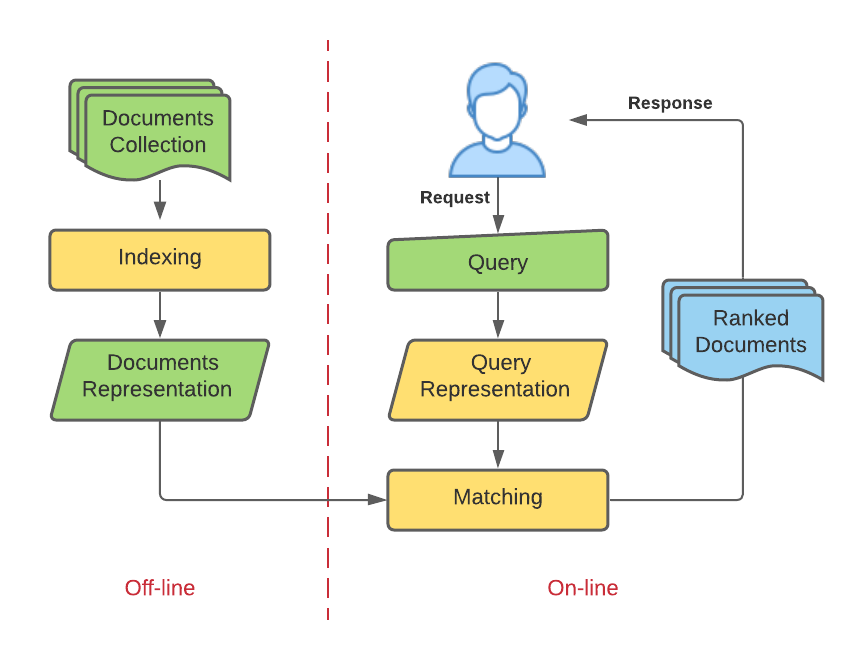
\includegraphics[width=0.8\linewidth]{images/irsystem.png}
  \caption{Schema di un sistema di information retrieval.}
\end{figure}

Un sistema di information retrieval è basato su un modello matematico che fornisce una descrizione formale del documento, della query e
di come comparare le rappresentazioni della query e del documento per stimare la rilevanza.

L'indicizzazione è un processo basato sull'estrazione di elementi (feature) che descrivono (rappresentano) il documento.
Nel caso di testi gli elementi sono generalmente parole e sono prendono il nome di indici.

Il matching può essere:
\begin{itemize}
  \item Esatto (binario): rilevante o non rilevante
  \item Parziale (graduale): la comparazione tra le rappresentazioni ha una certa tolleranza ai mismatch.
\end{itemize}

Per gestire l'informazione in modo automatico bisogna considerare due fattori:
\begin{itemize}
  \item \textbf{Efficienza}: come l'informazione viene rappresentata e processata.
  \item \textbf{Efficacia}: il modo in cui l'informazione viene sintetizzata e come la rappresentazione mantiene il significato originale.
\end{itemize}

Per misurare l'efficienza di un sistema di information retrieval è possibile calcolare precision e recall per ogni query.

\begin{figure}[ht]
  \centering
  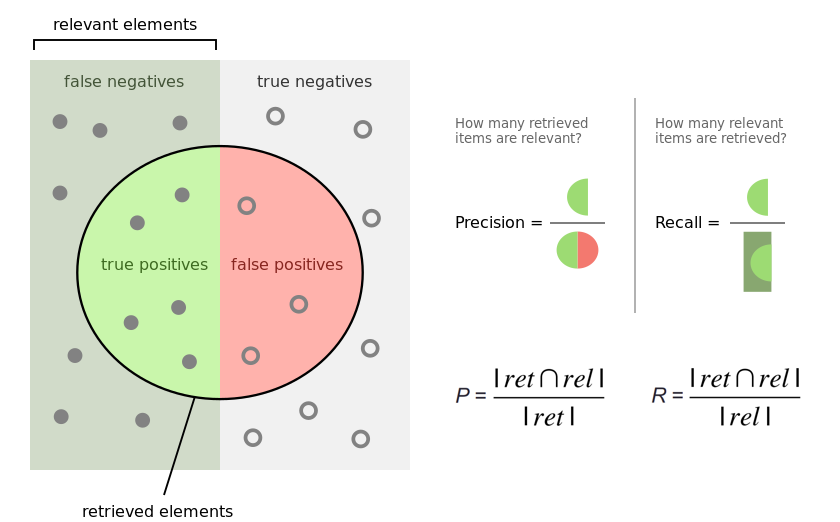
\includegraphics[width=\linewidth]{images/precisionrecall.png}
  \caption{Rappresentazione di precision e recall \cite{wiki:PrecisionRecall}.}
\end{figure}
\bigskip

\begin{quote}
  “IR must try to satisfy information needs expressed in a
  vague, inaccurate way through the ambiguities of the
  natural language, and must compare them, in an
  approximate way with the information contained in a
  document, and expressed through the same natural
  language”\par\nobreak\smallskip\hfill --- Smeaton, 1997
\end{quote}

L'information retrieval è caratterizzata da:
\begin{itemize}
  \item \textbf{Incompletezza} nella rappresentazione dei documenti
  \item \textbf{Soggettività} nel concetto di rilevanza
  \item \textbf{Ambiguità} nel significato dei termini
  \item \textbf{Vaghezza} nelle richieste dell'utente
  \item \textbf{Incertezza} della correttezza dei risultati
  \item \textbf{Approssimazione} del meccanismo di matching
\end{itemize}

\section{Data Structures}
L'indexing automatico di un documento testuale è un processo che mira ad associare gli indici a un testo.

L'uso di indici rende la ricerca di informazioni più efficiente basandosi sulle keyword specificate da una query.

L'insieme di tutti gli indici estratti da tutti i documenti della collezione costituiscono il \textbf{dizionario} della collezione.

Una volta estratti, gli indici vanno organizzati con una struttura dati con l'obiettivo di avere un accesso più efficiente possibile.

\subsection{Inverted File Structure}
Gli indici del dizionario vengono memorizzati e organizzati in un file chiamato \textbf{dictionary}. Ogni termine
punta a una lista (\textbf{posting list}) che contiene le reference ai documenti di cui il termine è un indice.
Le posting list sono memorizzate in un file a parte chiamato \textbf{posting file}.

% TODO: add image Dictionary e Posting File

Il dictionary contiene per ogni indice:
\begin{itemize}
  \item termine
  \item frequenza globale (nella collezione)
  \item puntatore alla posting list nel posting file
\end{itemize}

La posting list può contenere per ogni elemento:
\begin{itemize}
  \item identificatore univoco per il documento (DocID) che è associato ad un URI
  \item frequenza del termine nel documento (tf)
  \item posizione nel documento di ogni occorrenza del termine
\end{itemize}

Lo spazio richiesto dal dizionario è $O(\text{n}^\beta)$, dove n è lo spazio occupato dal testo dei documenti
e $\beta$ è una costante tra 0.4 e 0.6.

Lo spazio richiesto per memorizzare il numero di occorrenze è maggiore $O(n)$ perché ogni termine nel testo è referenziato
una volta nella struttura dato.

\subsection{Posting File Optimization}

\subsubsection*{DocID Compression}
La lista di DocID viene ordinata in ordine crescente e ogni $\text{DocID}_i$ viene rimpiazzato dalla differenza
$\text{DocID}_i - \text{DocID}_{i-1}$. I numeri ottenuti richiedono meno bit per essere codificati e permettono di ottenere una
riduzione del 10-15\% di spazio.

\subsubsection*{Block Division}
Il testo di ogni documento viene diviso in blocchi e la posizione delle occorrenze viene puntata al blocco.
Il numero di bit per codificare il puntatore sarà più piccolo del numero richiesto per le occorrenze nel punto esatto del testo.

Le ricerche contestuali però richiedono più operazioni.

\subsection{Dictionary Organization}

\subsubsection*{Linear Structure}
I termini sono memorizzati in ordine alfabetico.

\begin{itemize}
  \item accesso veloce con binary search $O(\log n)$
  \item memorizzazione efficiente
  \item adatto per la valutazione sequenziale
  \item per aggiungere nuovi termini bisogna ricostruire la struttura
\end{itemize}

\subsubsection*{Binary Tree Structure}
I termini sono memorizzati in un albero binario.
Ogni nodo ha due figli che separano gli indici a metà nell'ordine lessicografico.

La ricerca parte dalla radice e a ogni nodo viene scelto un figlio finché non si arriva al termine esatto.

\begin{itemize}
  \item accesso veloce con binary search $O(\log n)$
  \item la struttura va bilanciata se vengono aggiunti o rimossi dei termini
\end{itemize}

\subsubsection*{B-Tree Structure}
I termini sono memorizzati in un albero binario bilanciato di ordine $d$.
Ogni nodo ha un numero variabile di figli e contiene un massimo di $d$ termini e puntatori ai sotto-alberi.

La radice contiene un numero di termini tra 1 e $d$, mentre tutti gli altri nodi possono contenere un numero tra $d/2$ e $d$.

\begin{itemize}
  \item la ricerca ha tempo $O(\log_d n)$ dove $n$ è l'altezza dell'albero
  \item i termini possono essere aggiunti velocemente
  \item memorizzazione efficiente
  \item inefficiente per le ricerche sequenziali
  \item può diventare sbilanciato quando $n$ cresce.
\end{itemize}

\subsection{Altre Strutture di Indicizzazione}
% TODO

\section{Models}

\begin{itemize}
  \item set-based: boolean model, fuzzy model
  \item algebraic: VSM, generalized VSM, latent semantic indexing
  \item probabilistic: belief networks, language models
\end{itemize}

\subsection{Boolean Model}
Un documento è formalmente rappresentato da un insieme di indici.

Per ogni documento $d_j$ associamo ad ogni indice $t_i$ un peso binario $w_{ij} \in \{0, 1\}$ .
%
\begin{align*}
  R(d_j) = \{ t_i | w_{ij} = 1 \}
\end{align*}
%
La rappresentazione dei documenti viene invertita e associata ai termini.

\begin{table}[ht]
  \centering
  \begin{tabular}{lcl}
    $R(d_1) = \{t_1, t_2, t_3\}$ & $\rightarrow$ & $R(t_1) = \{d_1, d_2\}$ \\
    $R(d_2) = \{t_1, t_4, t_5\}$ & $\rightarrow$ & $R(t_2) = \{d_1, d_3\}$ \\
    $R(d_3) = \{t_2, t_5\}$      & $\rightarrow$ & $R(t_3) = \{d_1\}$
  \end{tabular}
\end{table}

Esempio delle operazioni di exact matching:

\begin{table}[ht]
  \centering
  \begin{tabular}{lcl}
    $q = t_1$           & $\rightarrow$ & $R(t_1) = \{d_1, d_2\}$                  \\
    $q = t_1 \land t_2$ & $\rightarrow$ & $R(t_1) \cap R(t_2) = \{d_1\}$           \\
    $q = t_1 \lor t_2$  & $\rightarrow$ & $R(t_1) \cup R(t_2) = \{d_1, d_2, d_3\}$ \\
    $q = \neg t_1$      & $\rightarrow$ & $C - R(t_1) = \{d_3\}$
  \end{tabular}
\end{table}

Una query viene rappresentata formalmente da un'espressione booleana di termini.

Ogni query può essere riscritta in forma normale disgiuntiva e ogni congiunzione rappresenta un
insieme di documenti ideali.

Una query è soddisfatta da un documento se appartiene a uno dei documenti ideali identificati da una congiunzione.
%
\begin{align*}
   & q = t_a \land (t_b \lor \neg t_c)                                                                                 \\
   & q_{dnf} = (t_a \land t_b \land t_c) \lor  (t_a \land t_b \land \neg t_c) \lor (t_a \land \neg t_b \land \neg t_c)
\end{align*}
%
L'ordine di valutazione di una query è importante, per questo è stata decisa una priorità degli operatori.
%
\begin{align*}
  lowest \qquad \text{OR} \quad \rightarrow \quad \text{AND, NOT} \quad \rightarrow \quad \text{ADJ, NEAR} \qquad highest
\end{align*}
%
Il matching mechanism applica delle operazioni insiemistiche.

La rilevanza è modellata come una proprietà booleana.
